\problemname{Ping Pong Tournament}
\noindent

Rulls is a true enthusiast of PO (the Pingis Olympiad).  
He loves following the matches and cheering on his favorite players as they compete.

PO is a table tennis tournament with an exciting format.  
The tournament begins with $N$ players, where each player has a starting position.  
Based on the starting positions, the players are paired up for matches.  
Each match results in a winner and a loser.  
The loser is eliminated and no longer plays any matches,  
while the winner advances to face the winner of another match.  
This process is repeated until only one player remains.

The tournament format can be illustrated with a tree diagram.

\begin{centering}
  \begin{figure}[h]
      \centering
      
\includegraphics[scale=0.7]{2.png}
    \caption{The diagram shows how the tree diagram of the tournament format looks for 4 players. The placement of the starting positions for the players is also a solution for sample 1.}
  \end{figure}
\end{centering}

During the first match, the player in the first position will play against the player in the second position, the player in the third position will play against the player in the fourth position, and so on.
The winner of each pair advances and will be paired up in a similar way.

To prevent the organizers from having to deal with troublesome situations, it is guaranteed that the number of players is always a power of two.

Now, PO is over for this season,  
but Rulls has forgotten which matches were played  
and which starting positions each player had.  
However, he remembers the number of matches each player won.

Given the number of wins for the $N$ players,  
output a possible order of the starting positions for the $N$ players.

Rulls remembers, however, that the starting positions were arranged in the lexicographically smallest possible order.
To get full points, you must find the lexicographically\footnote{https://en.wikipedia.org/wiki/Lexicographical\_order} smallest possible starting position.

A solution $A$ is lexicographically smaller than another solution $B$ if the following two conditions are met:  
\begin{enumerate}  
    \item $A \neq B$.  
    \item At the first position where $A$ and $B$ differ, the element in $A$ is smaller than the element in $B$.  
\end{enumerate}  

For example, if we have two solutions:  
$$
A = [1, 2, 4, 3], \quad B = [1, 3, 2, 4],  
$$  
the first position where $A$ and $B$ differ is position 1. There, $A[1] = 2$ and $B[1] = 3$. Since $2 < 3$, $A$ is lexicographically smaller than $B$.  


\section*{Input}
The first line contains an integer $N$ ($1 \leq N \leq 2^{19}$), the number of players in the tournament. $N$ is guaranteed to be a power of two.

The second line contains $N$ integers, where $a_i$ ($0 \leq a_i \leq 10^9$ for all $1 \leq i \leq N$) is the number of matches that the $i$-th player won during the tournament.

\section*{Output}
Output $N$ integers, a permutation of the integers $1, 2, \ldots, N$, where the permutation represents the starting positions in the tournament.  
To get full points, you must also output the lexicographically smallest permutation.

If it is impossible to find starting positions for these $N$ players, output $-1$.

\section*{Scoring}
Your solution will be tested on a set of test groups, each worth a number of points. Each test group contains
a set of test cases. To get the points for a test group you need to solve all test cases in the test group.
For each test group, if your program answers correctly whether it is possible or not,  
and outputs a valid permutation of starting positions, you will receive \underline{\textbf{50\%}} of the points for that test group.

To earn all the points in a test group, you must output the lexicographically smallest permutation.

\noindent
\begin{tabular}{| l | l | p{12cm} |}
  \hline
  \textbf{Group} & \textbf{Points} & \textbf{Constraints} \\ \hline
  $1$    & $2$        & $N \leq 2$ \\ \hline
  $2$    & $6$        & $N \leq 4$ \\ \hline
  $3$    & $12$       & $N \leq 8$ \\ \hline
  $4$    & $18$       & $N \leq 2^7 = 128$ \\ \hline
  $5$    & $12$       & $N \leq 2^{11} = 2048$ \\ \hline
  $6$    & $12$       & $a_i \leq a_{i+1}$ for all $1 \leq i \leq N-1$. \\ \hline 
  $7$    & $38$       & No additional constraints. \\ \hline % N <= 2^19 ≈ 5*10^5 or 2^18 ≈ 2*10^5
\end{tabular}


\section*{Explanation of Samples}
In the first sample, one possible solution is for the players to start at the bottom of the tournament in the order $[1, 3, 2, 4]$. While $[1, 4, 2, 3]$ is also a valid solution, the former is lexicographically smaller.
Note that player $1$ will play a ping-pong match against player $3$, but since we know that player $3$ lost all of their matches, player $1$ must have won that match.

\begin{centering}
  \begin{figure}[h]
      \centering
      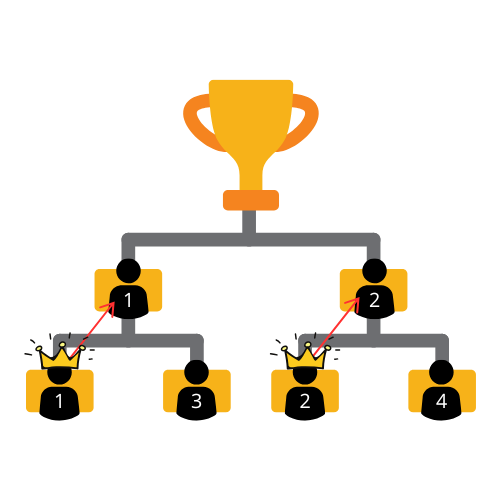
\includegraphics[scale=0.7]{4.png}
    \caption{By placing the players according to the starting positions $[1, 3, 2, 4]$ in sample 1, player 1 and player 2 win their first matches.}
  \end{figure}
\end{centering}

\begin{centering}
  \begin{figure}[h]
      \centering
      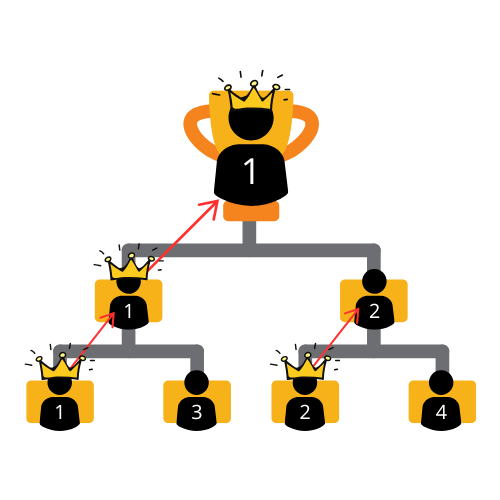
\includegraphics[scale=0.7]{6.png}
    \caption{Player 1 then wins the final match, thus fulfilling the input requirements.}
  \end{figure}
\end{centering}


In the second sample, it is impossible for all players to win exactly one match. Therefore, the output is ``-1''.
